\section{Related Work}

Researchers have long realized that incomprehensible type errors result as a consequence of standard approaches to the type inference process. Haack and Wells~\cite{haack2004type} noted that ``\textit{Identifying only one node or subtree of the program as the error location makes it difficult for programmers to understand type errors. To choose the correct place to fix a type error, the programmer must find all the other program points that participate in the error.}'' Researchers have proposed solutions to improve the type inference process. Type error slicing~\cite{haack2004type} is a technique that finds locations that are complete and minimal for the type error. Internally labeled constraints and MUS manipulation are used to generate these slices. The language supported in Haack's work was a subset of standard ML. The original Chameleon~\cite{stuckey2003interactive} used a similar technique but extended it to support advanced type-level features (type classes and functionally dependent types). The project also introduced the ability to query type information through a command line-style interface (Fig.~\ref{fig:original-chameleon}). Although Chameleon was firmly grounded in results from type theory, its designs were never evaluated with user studies.

Another direction to approach type error debugging is suggesting fixes. Sheng Chen's works [1,2] on counter factual typing is able to suggesting changes to make the ill-typed program typecheck. While this is promising ground, the work is not evaluated with human participants.  \cite{lerner2007searchingtypeerror} used an approach by repeatedly modifying the abstract syntax tree and querying the compiler/type checker to know whether the program still well-typed. This approach allows the algorithm to produce suggestions the syntax changes that could fix the type error. Benefiting from not needing a type system impelemntation and being language agnositic, the underlying idea was implemented and evaluated on 10 CS students. The system can be successfully adopted in not suitable for teaching and learning purpose, as it is not able to explain why the type error happened and why fixes are suggested. The lack of explanability is because the information was witheld by the type checker and the inference algorthm does not know (need to know) how types are computed.

One related approach is CEME (compiler error message enhancement). Prather showed that ECEM casts a positive result in understanding the type error through a series of mixed methods study. Decafe is a tool that is able to rephase the compier error message into an enhanced version. A study of over 200 CS1 students showed that CEME reduce overall errors in their assignments. Berik proposed a framework of constructing compiler error message based on the augumentation theory. In this proposal,  Berik argued that error messages  follow a simple argumentation layout or an exntended argumentation layout will result in a human friendly errors.  These research shows the significance of improving the language in a compiler error message. Most principles and suggestions are followed in \chameleon{} in concustructing error statements. However they were not targeting type errors but compiler error (some even include runtime error) in general. The nuances of type errors, such as alternative typings were not taken into account. 

% \begin{figure}[h]
%     \centering
%     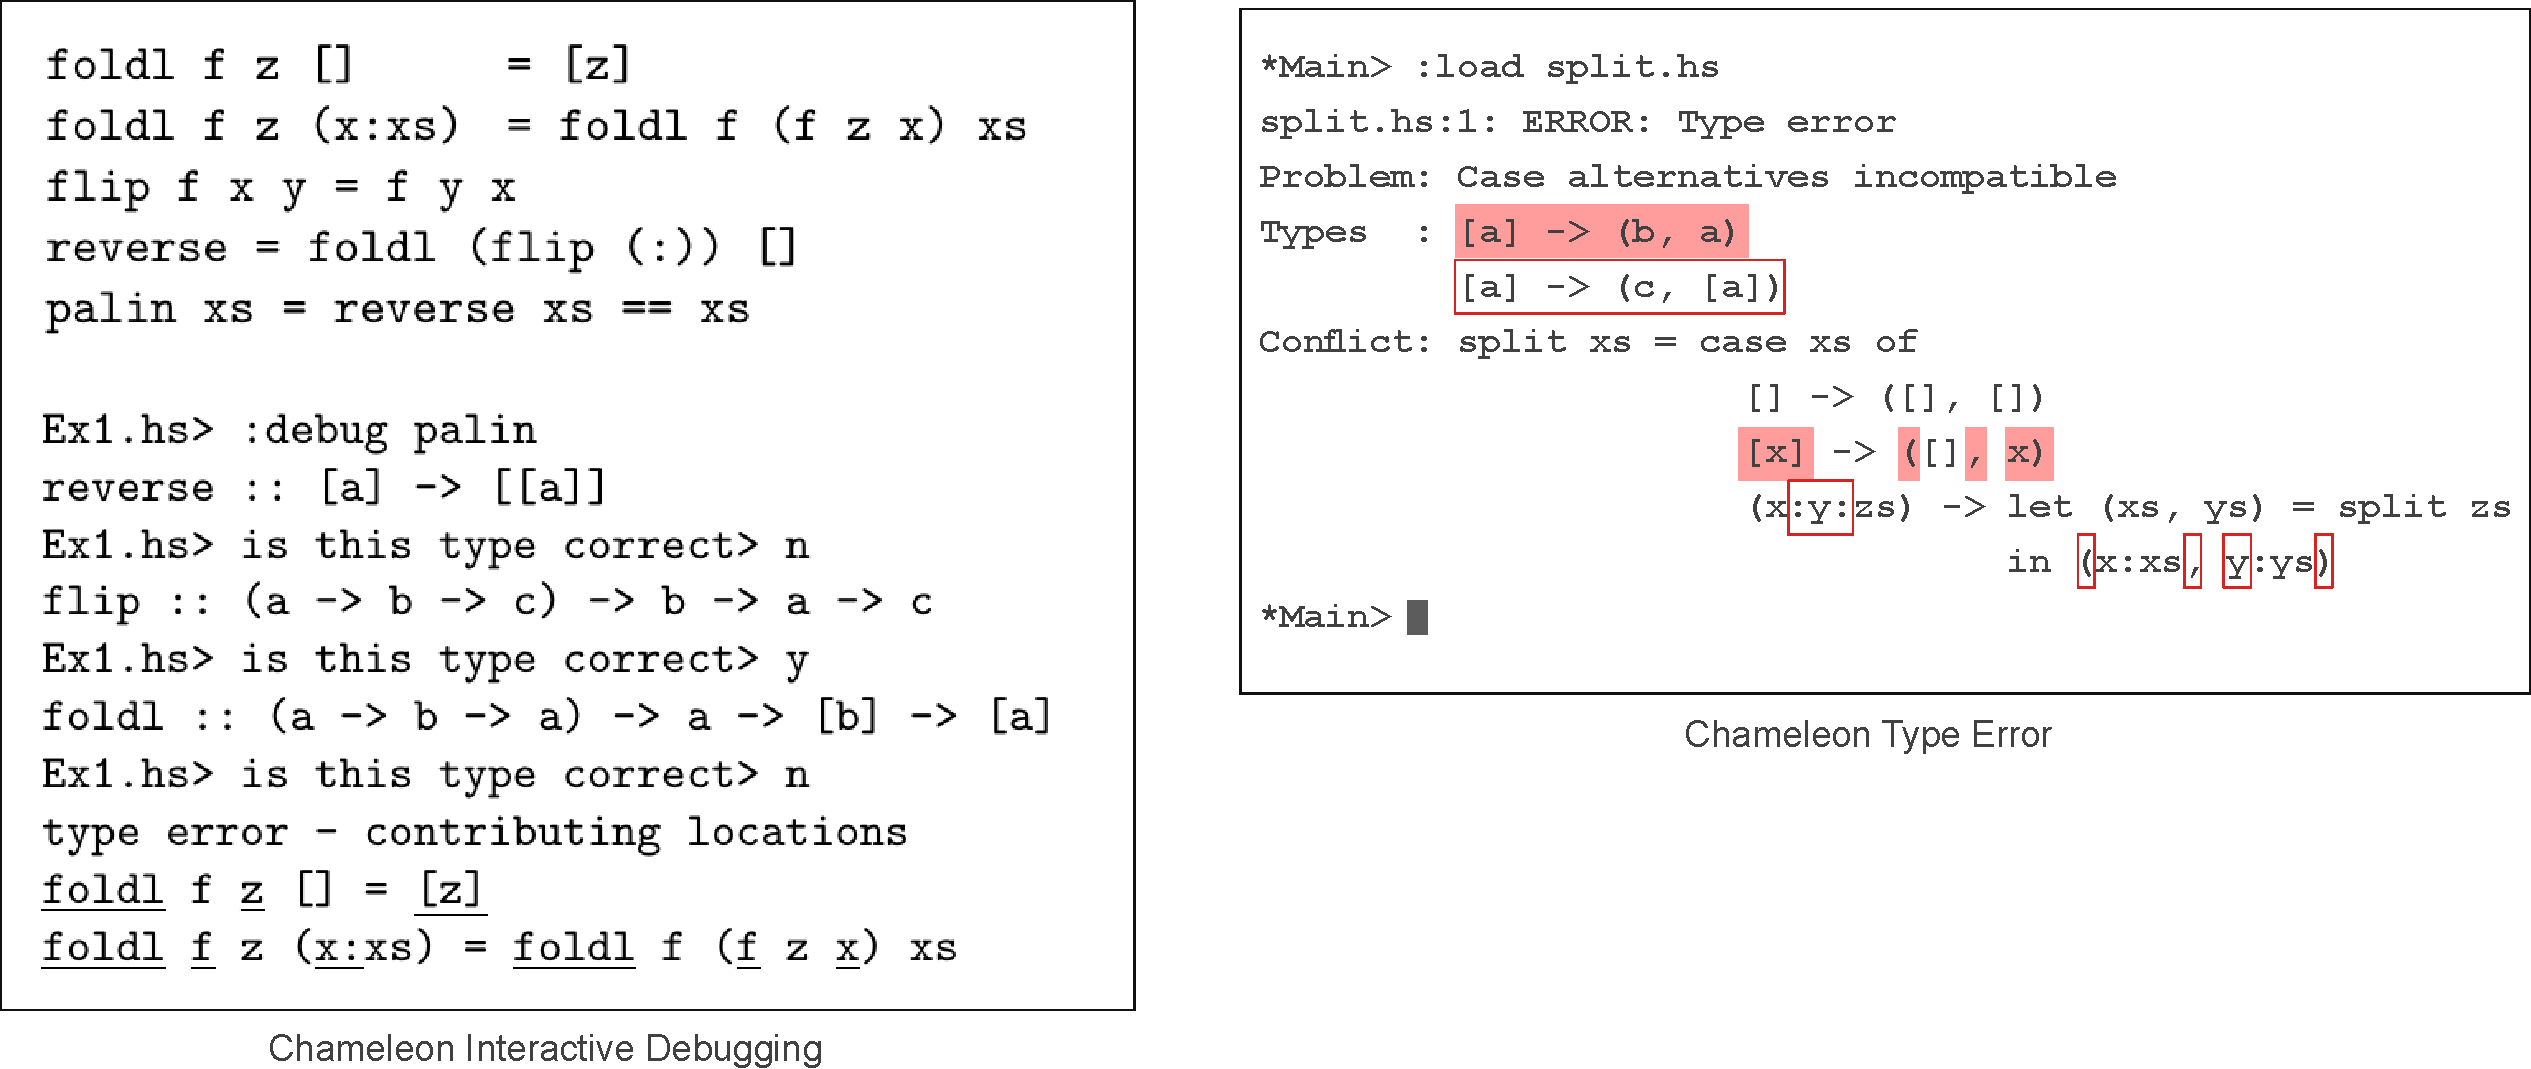
\includegraphics[width=\linewidth]{images/original-chameleon.pdf}
%     \caption{
% Originally, Chameleon was a command-line tool that can list all the potential causes of a type error and display the two branches in two forms of highlight (right), achieved with ASCII colors. In addition, it allows a few commands (debug and explain) in the debugging shell to help debug type errors (left).}
%     \label{fig:original-chameleon}
% \end{figure}


% The ChameleonIDE error reporting The error message of ChameleonIDE closely
% follows the argumentation structure outlined by Titus. Basic mode represent a
% simple structure argument, where the claim "The expression e can have two
% conflicting types" and the possible type 1 and two serves as grounds. When
% inspecting each possible types, the type judgements are treated as claim, and it
% is supported by the grounds: "Inferred from the orange/blue highlights on the
% left side". On the other hand, the similar type error message in GHC "Couldn't
% match expect type T1 with actual type T2" is "a ground masquerading as a clam",
% Barik commented. The balanced mode and advanced mode serve as a way to elaborate
% arguments from simple arguments into extended arguments.

% Another related topic is type-explanation~\cite{yang1999explaining, jun2002explaining}. Yang~\cite{jun2002explaining} showed an alternative type inference system capable of producing a human-like text explanation for why expressions are assigned certain types. A good explanation is drawn from surveying how human experts explain types. The resulting algorithm $\mathcal{H}$, generates a succinct explanation of the type inference steps to avoid using internal constructs (such as type variables). The explanation system has the advantage of acting like a human expert. However, when presented as text-based output, explanation systems have the potential to become verbose when types are complex or variable names are long. In \chameleon{}, we attempt to address this problem by showing one step of explanation at a time and referring to variables instead of spelling out the full name.




Debugging using a GUI Interactive Development Environment has been the standard practice for a very long time. Compared to a command line-based interface, a graphic user interface provides programming tools with the ability to show information hierarchy, provide immediate feedback to changes, and display complex visualizations. Provide opportunities to run consecutive command to query the information about code or executing command based on the existing code.
HazelTutor is a interactive filling type holes by suggesting template expressions (strategies as called by the authors). It also provide a cursor based type inspector that allows programmers to query the type of parts of the program.
Whyline~\cite{ko2009finding} is a Java debugging system that allows a user to ask questions like "why does variable X have value Y". It also allows users to interactively ask follow-up questions to gain further knowledge of the nature of an error.  These debugging tools are great motivations for the development of \chameleon{}. However they focus on different aspect of debugging. Java Whyline mainly tackle the problem of unintended runtime behavior while HazelTutor specialized in interactive actions supporting type holes.


